\documentclass{beamer}
\usepackage{default}
\usepackage{amsmath}
\usepackage{graphicx}
\usepackage{adjustbox}  % Allows for fitting tables into slide
\usepackage{hyperref}
\usepackage{threeparttable}
\usepackage{caption}
%\usepackage{subcaption}
\usepackage{natbib}
\usepackage{adjustbox}
\usepackage{subcaption}




%\usetheme{AnnArbor}
%\usetheme{Antibes}
%\usetheme{Bergen}
%\usetheme{Berkeley}
%\usetheme{Berlin}
%\usetheme{Boadilla}
%\usetheme{boxes}
\usetheme{CambridgeUS}
%\usetheme{Copenhagen}
%\usetheme{Darmstadt}
%\usetheme{default}
%\usetheme{Frankfurt}
%\usetheme{Goettingen}
%\usetheme{Hannover}
%\usetheme{Ilmenau}
%\usetheme{JuanLesPins}
%\usetheme{Luebeck}
%\usetheme{Madrid}
%\usetheme{Malmoe}
%\usetheme{Marburg}
%\usetheme{Montpellier}
%\usetheme{PaloAlto}
%\usetheme{Pittsburgh}
%\usetheme{Rochester}
%\usetheme{Singapore}
%\usetheme{Szeged}
%\usetheme{Warsaw}

% colortheme to choose one 

%\usecolortheme{beaver}
%\usecolortheme{crane}
%\usecolortheme{default}
\usecolortheme{dolphin}
%\usecolortheme{seagull}
%\usecolortheme{seahorse}
%\usecolortheme{whale}


% fond theme to choose one 
%\usefonttheme{structuresmallcapsserif}
%\usefonttheme{structureitalicserif}
%\usefonttheme{structurebold}
\usefonttheme{serif}
%\usefonttheme{professionalfonts}
%\usefonttheme{default}

\title{Perceived Income Risks}


% A subtitle is optional and this may be deleted

\author{Tao Wang \\ Johns Hopkins University}
% - Give the names in the same order as the appear in the paper.
% - Use the \inst{?} command only if the authors have different
%   affiliation.

\date{\today}
% - Either use conference name or its abbreviation.
% - Not really informative to the audience, more for people (including
%   yourself) who are reading the slides online

% This is only inserted into the PDF information catalog. Can be left
% out. 

% If you have a file called "university-logo-filename.xxx", where xxx
% is a graphic format that can be processed by latex or pdflatex,
% resp., then you can add a logo as follows:

% \pgfdeclareimage[height=0.5cm]{university-logo}{university-logo-filename}
% \logo{\pgfuseimage{university-logo}}

% Delete this, if you do not want the table of contents to pop up at
% the beginning of each subsection:
\AtBeginSubsection[]
{
	\begin{frame}<beamer>{Outline}
	\tableofcontents[currentsection]
\end{frame}
}

\begin{document}
	

\begin{frame}
	\titlepage
\end{frame}
\begin{frame}{Outline}
	\tableofcontents
	% You might wish to add the option [pausesections]
\end{frame}


\section{Motivation}

\begin{frame}{Motivation}
	\begin{itemize}
		\item Not just expectation of income but also \textcolor{blue}{high moments} such as income risks matter for consumption/portfolio decisions, i.e. precautionary motives, stock market investment, etc. 
		\item \textcolor{blue}{Uninsurance} of idiosyncratic risks make it matter in macroeconomics working assumption by the HANK literature  
		\item It is pepple's perceptions that directly drive that decisions
		\item Are the perceptions in line with econometricians' estimates of income risks based on cross-sectional inequality and the size of income income risks used in heterogeneous macro?
	\end{itemize}
\end{frame}


\begin{frame}{This paper's agenda}
	\begin{enumerate}
		\item Using density survey of labor income to directly shed light on perceived risk profile
		\begin{itemize}
			\item Perceived income risks differ systematically across age, generations, genders and education. 
			\item Evidence of non-normality, i.e half of the sample have non-zero skewness
			\item Perceived risks and skewness negatively correlate with stock market returns.  
		\end{itemize}
		\item Characterize the potential differences between perceptions, econometrician's estimates used in structural model so far. 
		\begin{itemize}
		    \item Do people understand the permanent and transitory risks perfectly?
		\end{itemize}
		\item Incorporating \textcolor{blue}{imperfect understanding} of income process into an otherwise standard heterogenous-agent model featuring uninsured idiosyncratic risks 
\end{enumerate}
\end{frame}


\begin{frame}{Literature}
\begin{itemize}
	\item ``insurance or information'': \cite{pistaferri_superior_2001}, \cite{kaufmann_disentangling_2009}, \cite{meghir2011earnings}, \cite{flavin_excess_1988}, New York Fed Blog (2019) 
   \item consumption/saving and portfolio choice incorporating imperfect perception/understanding. \cite{rozsypal_overpersistence_2017}, \cite{carroll_sticky_2018}, \cite{lian2019imperfect}.  
   \item expectation formation, mostly on macroeconomic variables, \cite{coibion2012can}, \cite{fuhrer2018intrinsic}, etc. 
   \item subjective survey, especially on probabiblist surveys.  \cite{manski_measuring_2004}, \cite{delavande2011measuring}, \cite{manski_survey_2018}, \item \cite{bertrand_people_2001}, \cite{armantier_overview_2017}
   \item Heterogeneous agent macro (HANK): uninsured idiosyncratic risks leads to ex post heterogeneity. \cite{xxx}
   \item Long-run risk \cite{xxx} 
  \end{itemize}
\end{frame}

\section{Stylized facts}


\begin{frame}{Data}
	\begin{table}
		\centering
		\caption{Survey of Consumer Expectations}
		\label{SCE_data_sum}
		\adjustbox{max height=0.5\textheight, max width=\textwidth}{ 
			\begin{tabular}{lll}
				\hline 
				Time period                                    & 2013M6-2019M6           \\
				Frequency                                      & monthly                                 \\
				Sample size                                    & 1,300                                  \\
				Density variable                    &  \textcolor{blue}{1-yr-ahead earning growth   (same position/hours) }           \\
				Pannel structure                               & stay up to 12 months      \\
				Demographics                     & educ, income, age        \\
				\hline 
			\end{tabular}
		}
	\end{table}
	\begin{itemize}
		\item density estimation following (\cite{engelberg_comparing_2009})
		\item exclude top and bottom 5\% values for forecast errors and uncertainty
	\end{itemize}
\end{frame}


\begin{frame}{Definitions}
	\begin{itemize}
		\item Moments to look at 
		\begin{itemize}
			\item expected growth, $E_i (\Delta y_i)$
			\item variance: $\overline {var}_i(\Delta y_i)$
			\item skewness: $\overline {skew}_i(\Delta y_i)$
		\end{itemize}
		\item Both pereived nominal and real income growth 
		\begin{itemize}
			\item $E_i(\Delta y^r_i) =E_i(\Delta y_i^n) - E_i(\pi)$
			\item $\overline{var}_i(\Delta y_i^r) =\overline {var}_i(\Delta y_i^n) +  \overline {var}_i(\pi)$
		\end{itemize}
		\item Conditional on employment.
		\begin{itemize}
			\item Can be adjusted to unconditional risk using perceived unemployment risk. So the perceived risk of same job/hour is just a lower bound for income risk. 
		\end{itemize}
	\end{itemize}
\end{frame}

\subsection{Cross-sectional patterns}

\begin{frame}{Cross-sectional distribution of expected income growth}
	\begin{figure}
	\centering
	\label{incexp_hist}
	\begin{subfigure}[b]{0.45\textwidth}
		\centering
		\caption{nominal income expectation}
		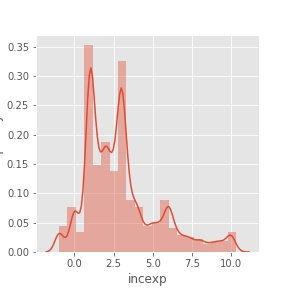
\includegraphics[width=\textwidth]{figures/hist_incexp}
	\end{subfigure}
	\begin{subfigure}[b]{0.45\textwidth}
		\centering
		\caption{real income expectation}
		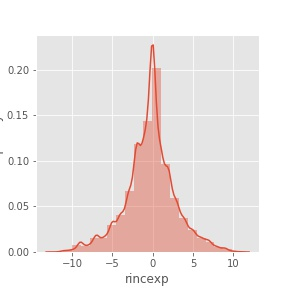
\includegraphics[width=\textwidth]{figures/hist_rincexp}
	\end{subfigure}
\end{figure}
	\begin{itemize}
		\item Nominal rigity can be seen from the expected norminal earning growth, while real expected growth become symmetric 
	\end{itemize}
\end{frame}

\begin{frame}{Cross-sectional distribution of income dispersion}
	\begin{figure}
		\centering
		\label{incvar_hist}
			\begin{subfigure}[b]{0.45\textwidth}
			\centering
			\caption{nominal income risk}
		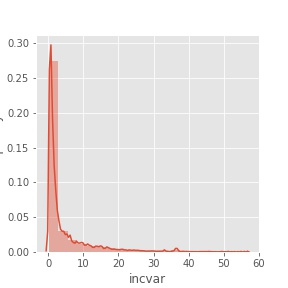
\includegraphics[width=\textwidth]{figures/hist_incvar}
		\end{subfigure}
		\begin{subfigure}[b]{0.45\textwidth}
		\centering
		\caption{real income risk}
		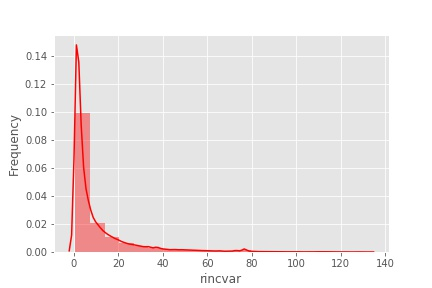
\includegraphics[width=\textwidth]{figures/hist_rincvar}
	\end{subfigure}
	\end{figure}
	\begin{itemize}
		\item average perceived income risks:  $3\%$ standard deviation for nominal and $4\%$ standard deviation for real income
		\item just a lower bound: before adjustment of unemployment risk 
	\end{itemize}
\end{frame}

\begin{frame}{Cross-sectional distribution of tail risks}
	\begin{figure}
	\centering
	\label{incskew_hist}
	\begin{subfigure}[b]{0.45\textwidth}
		\centering
		\caption{nominal income skewness}
		\includegraphics[width=\textwidth]{figures/histincSkew}
	\end{subfigure}
\end{figure}
	\begin{itemize}
		\item sizable dispersion in skewness, i.e. about half of the people have non-zero skewness in perceived inome distribution. 
	\end{itemize}
\end{frame}



\begin{frame}{Perceived income risks by household income}
	\begin{figure}[ht]
		\label{ts_incvar_HHinc_g_mean}
		\begin{subfigure}[b]{0.7\textwidth}
			\centering
			\caption{nominal income risks}
			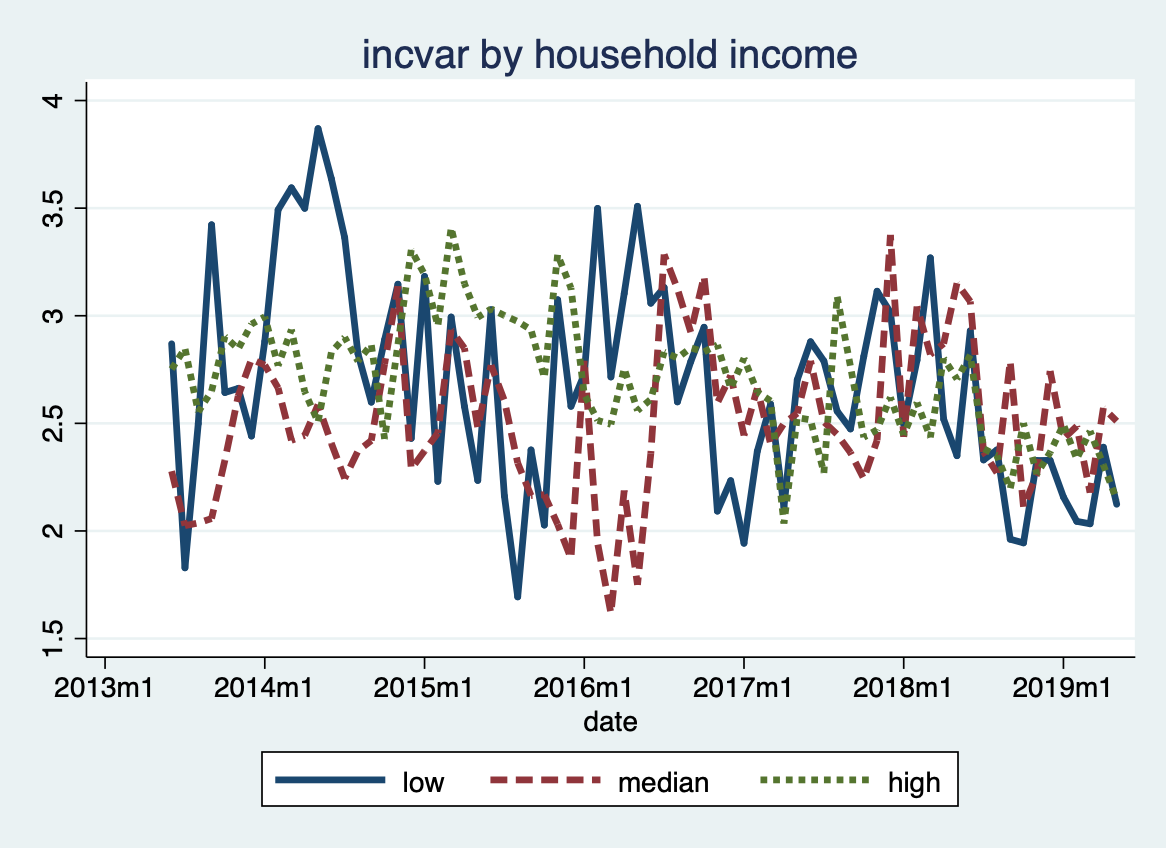
\includegraphics[width=\textwidth, height = 0.33\textheight]{figures/ts_incvar_HHinc_g_mean.png}
		\end{subfigure}
		\begin{subfigure}[b]{0.7\textwidth}
			\caption{real income risks}
			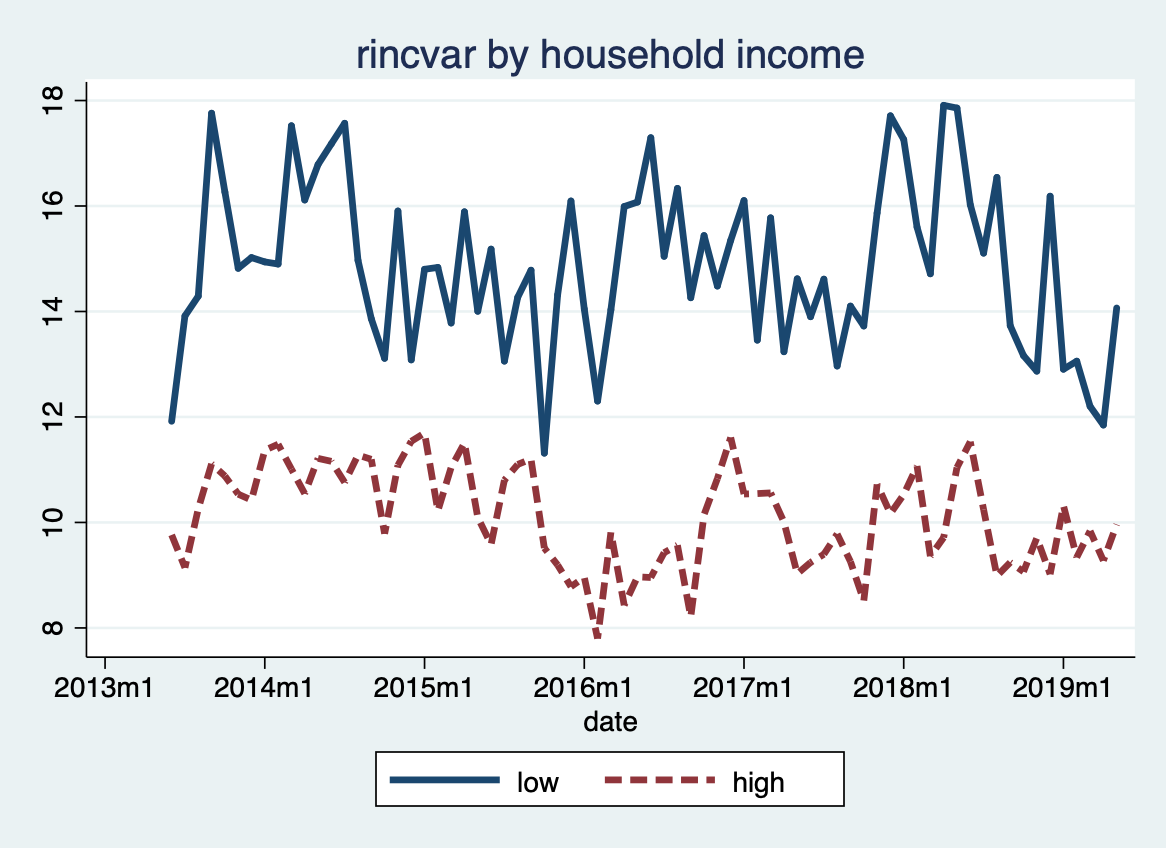
\includegraphics[width=\textwidth, height = 0.33\textheight]{figures/ts_rincvar_HHinc_g_mean.png}
		\end{subfigure}
	\end{figure}
\end{frame}


\begin{frame}{Perceived income risks by household income}
	\begin{figure}
		\centering
		\label{boxplot_hhinc}
		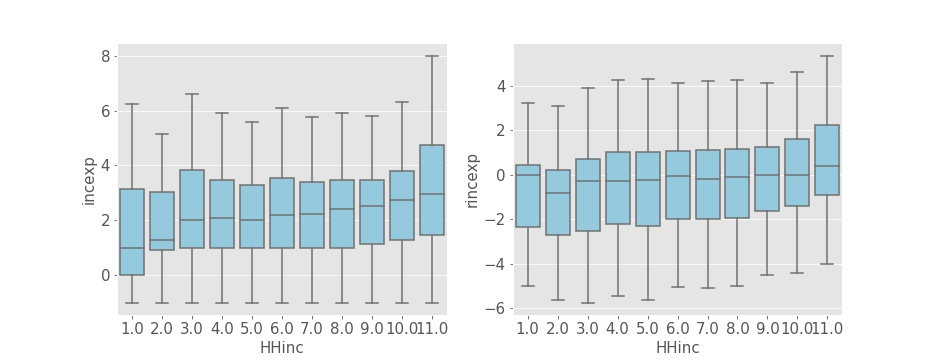
\includegraphics[width=0.8\textwidth]{figures/boxplot_exp_HHinc} \\
		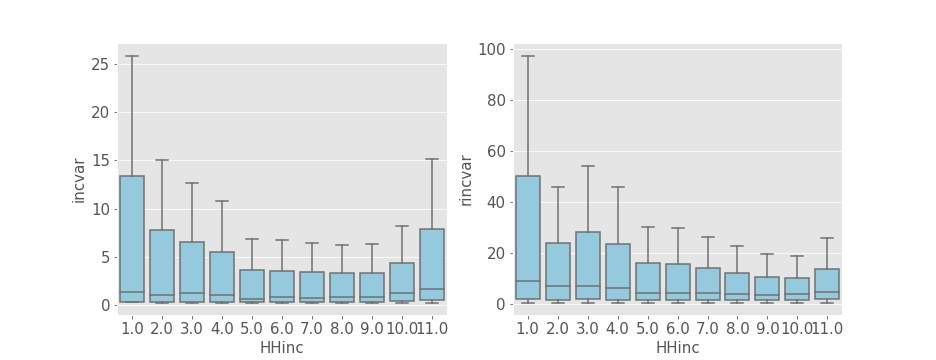
\includegraphics[width=0.8\textwidth]{figures/boxplot_var_HHinc}
	\end{figure}
	\begin{itemize}
		\item 
	\end{itemize}
\end{frame}



\begin{frame}{Perceived income risks by age}
	\begin{figure}[ht]
		\label{ts_incvar_age_g_mean}
		\begin{subfigure}[b]{0.7\textwidth}
			\centering
			\caption{nominal income risks}
			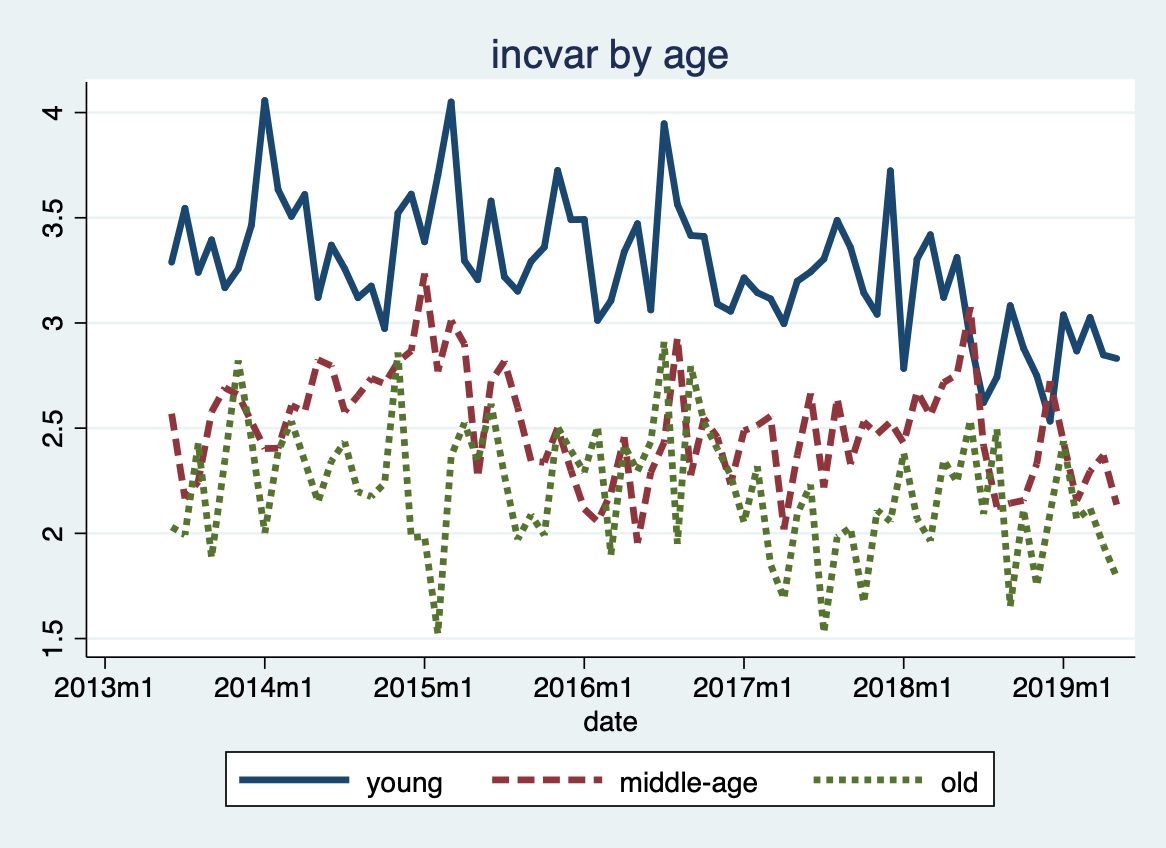
\includegraphics[width=\textwidth, height = 0.33\textheight]{figures/ts_incvar_age_g_mean.png}
		\end{subfigure}
		\begin{subfigure}[b]{0.7\textwidth}
			\caption{real income risks}
			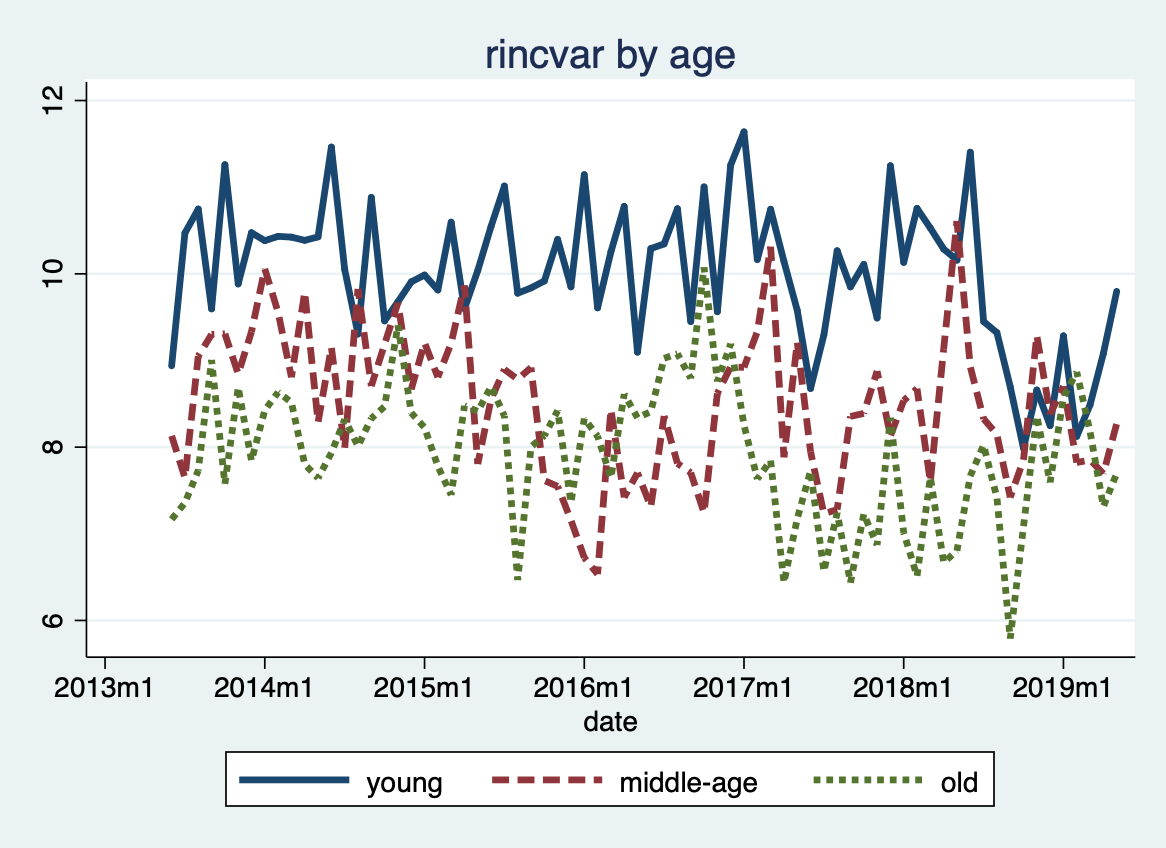
\includegraphics[width=\textwidth, height = 0.33\textheight]{figures/ts_rincvar_age_g_mean.png}
		\end{subfigure}
	\end{figure}
\end{frame}

\begin{frame}{Perceived income risks by age}
	\begin{figure}
		\centering
		\label{boxplot_age_gr}
		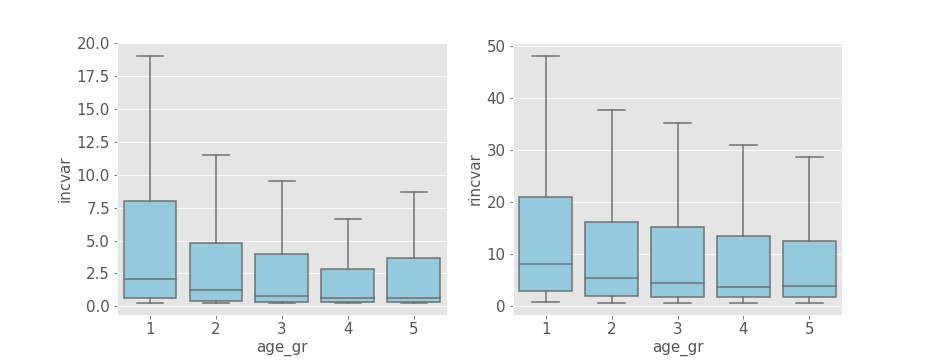
\includegraphics[width=0.8\textwidth]{figures/boxplot_exp_age_gr} \\
		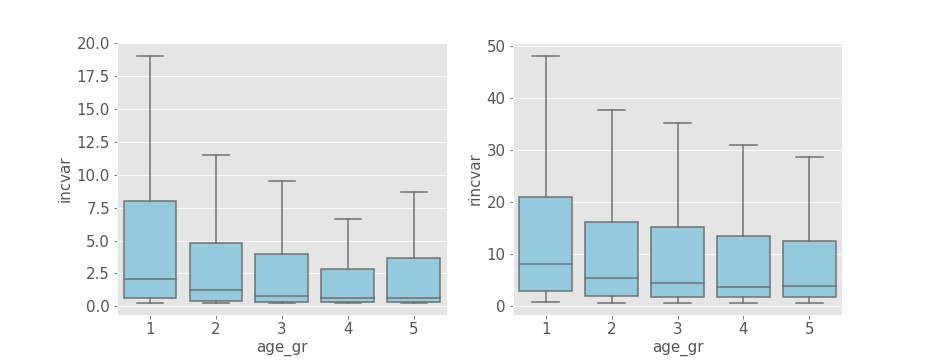
\includegraphics[width=0.8\textwidth]{figures/boxplot_var_age_gr}
	\end{figure}
	\begin{itemize}
		\item 
	\end{itemize}
\end{frame}


\begin{frame}{Perceived income risks by generation}
	\begin{figure}[ht]
		\label{ts_incvar_byear_g_mean}
		\begin{subfigure}[b]{0.7\textwidth}
			\centering
			\caption{nominal income risks}
			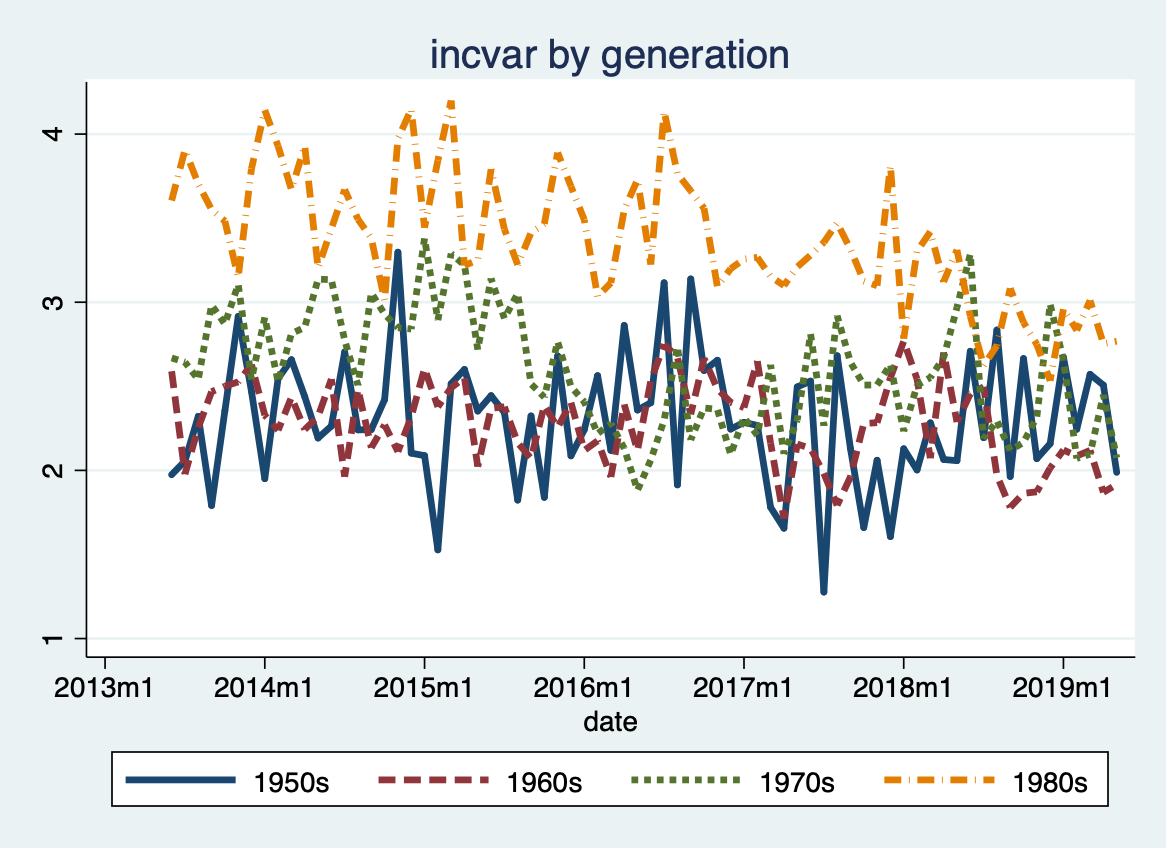
\includegraphics[width=\textwidth, height = 0.33\textheight]{figures/ts_incvar_byear_g_mean.png}
		\end{subfigure}
		\begin{subfigure}[b]{0.7\textwidth}
			\caption{real income risks}
			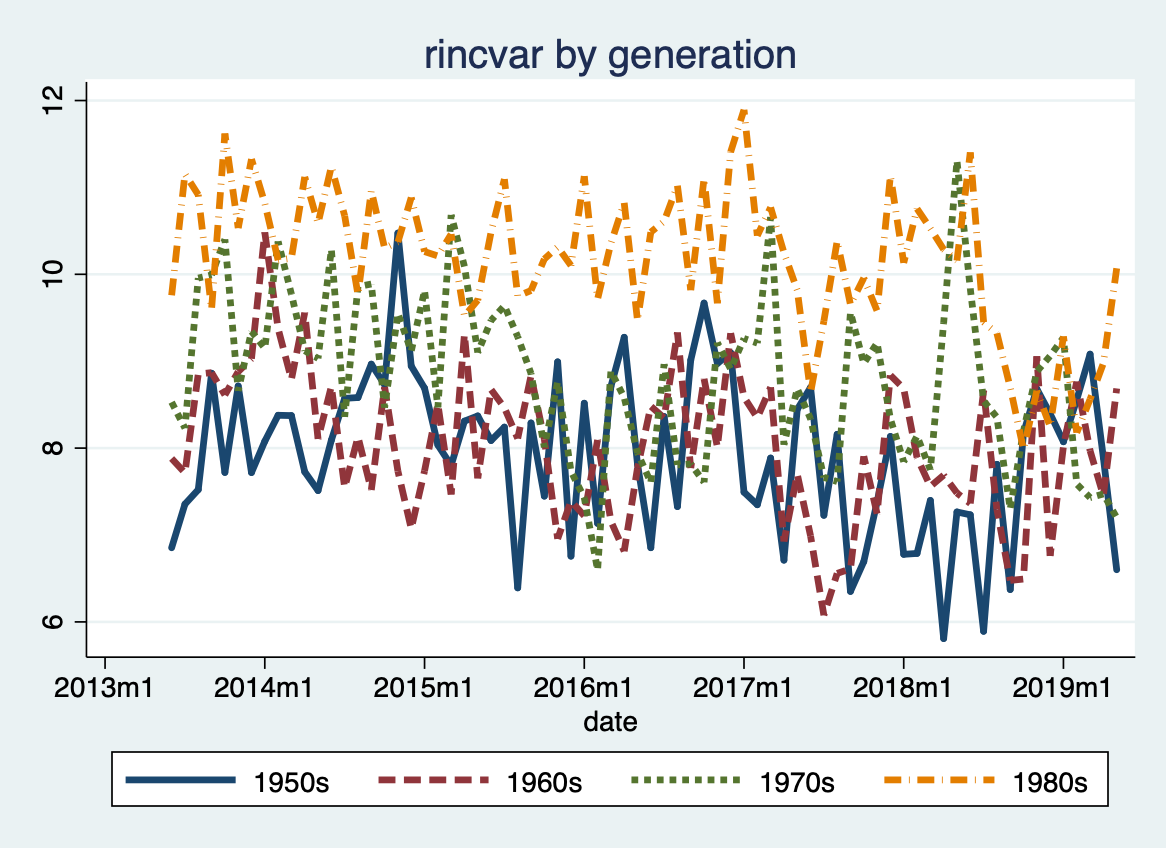
\includegraphics[width=\textwidth, height = 0.33\textheight]{figures/ts_rincvar_byear_g_mean.png}
		\end{subfigure}
	\end{figure}
\end{frame}


\begin{frame}{Perceived income risks by generation}
	\begin{figure}
		\centering
		\label{boxplot_byear_gr}
		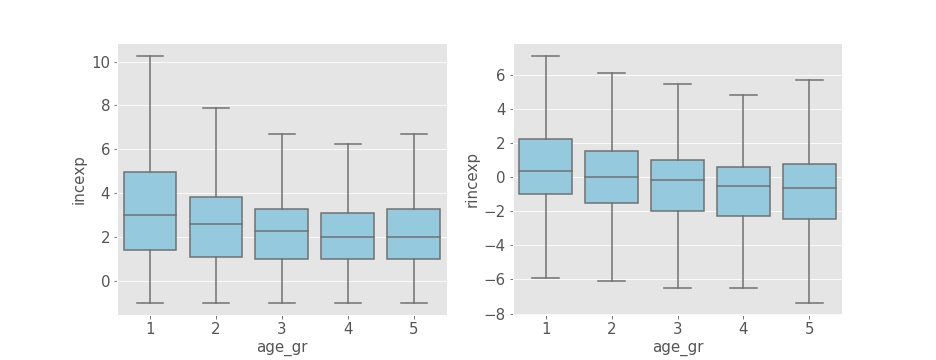
\includegraphics[width=0.8\textwidth]{figures/boxplot_exp_byear_gr} \\
		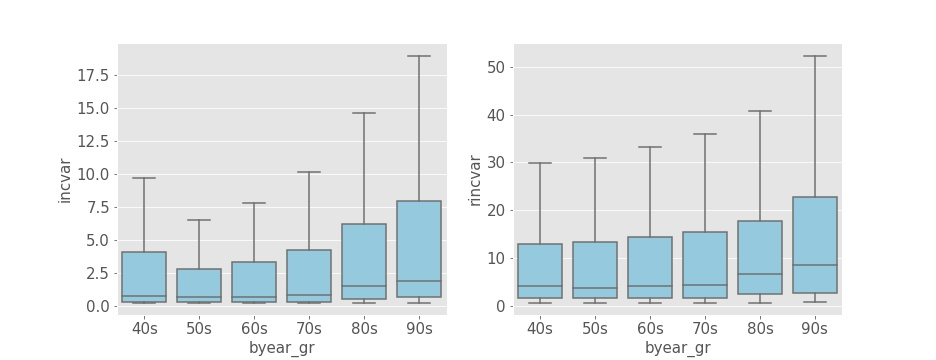
\includegraphics[width=0.8\textwidth]{figures/boxplot_var_byear_gr}
	\end{figure}
	\begin{itemize}
		\item 
	\end{itemize}
\end{frame}


\begin{frame}{Covariants of expected income growth}
	\begin{table}
		\centering
		\caption{Expected income growth and individual characteristics}
		\label{micro_reg_exp}
		\adjustbox{max height=0.5\textheight, max width=\textwidth}{ 
			\begin{tabular}{ccccccccc}
				\hline 
				{} &  incexp I & incexp II & incexp III & incexp IIII & rincexp I & rincexp II & rincexp III & rincexp IIII \\
				\hline 
				HHinc\_gr=low inc &           &           &      -0.03 &             &           &            &    -0.39*** &              \\
				&           &           &     (0.02) &             &           &            &      (0.03) &              \\
				educ\_gr=low educ &           &           &            &    -0.25*** &           &            &             &     -0.63*** \\
				&           &           &            &      (0.02) &           &            &             &       (0.03) \\
				gender=male      &           &           &            &    -0.32*** &           &            &             &     -0.78*** \\
				&           &           &            &      (0.02) &           &            &             &       (0.03) \\
				parttime=yes     &  -0.47*** &  -0.36*** &   -0.35*** &             &  -0.63*** &   -0.53*** &    -0.44*** &              \\
				&    (0.03) &    (0.03) &     (0.03) &             &    (0.04) &     (0.04) &      (0.04) &              \\
				selfemp=yes      &   0.86*** &  -0.00*** &    0.00*** &             &   0.84*** &   -0.00*** &    -0.00*** &              \\
				&    (0.03) &    (0.00) &     (0.00) &             &    (0.05) &     (0.00) &      (0.00) &              \\
				Stkprob          &           &   0.01*** &    0.01*** &             &           &    0.02*** &     0.02*** &              \\
				&           &    (0.00) &     (0.00) &             &           &     (0.00) &      (0.00) &              \\
				UEprobInd        &           &  -0.01*** &   -0.01*** &             &           &   -0.02*** &    -0.02*** &              \\
				&           &    (0.00) &     (0.00) &             &           &     (0.00) &      (0.00) &              \\
				Intercept        &   2.82*** &   2.57*** &    2.58*** &     3.05*** &  -0.29*** &   -0.92*** &    -0.80*** &      0.20*** \\
				&    (0.01) &    (0.02) &     (0.02) &      (0.02) &    (0.02) &     (0.03) &      (0.03) &       (0.02) \\
				\hline 
				N                &     54275 &     48606 &      48606 &       47712 &     49702 &      44446 &       44446 &        43694 \\
				R2               &      0.01 &      0.02 &       0.02 &        0.01 &      0.01 &       0.04 &        0.04 &         0.02 \\
				
				\hline 
			\end{tabular}
		}
	\end{table}
\end{frame}

\begin{frame}{Covariants of perceived income risks}
	\begin{table}
		\centering
		\caption{Perceived income risks and individual characteristics}
		\label{micro_reg}
		\adjustbox{max height=0.5\textheight, max width=\textwidth}{ 

\begin{tabular}{ccccccccc}
	\hline 
	{} & incvar I & incvar II & incvar III & incvar IIII & rincvar I & rincvar II & rincvar III & rincvar IIII \\
	\hline 
	HHinc\_gr=low inc &          &           &    1.56*** &             &           &            &     7.01*** &              \\
	&          &           &     (0.10) &             &           &            &      (0.19) &              \\
	educ\_gr=low educ &          &           &            &     0.40*** &           &            &             &      3.82*** \\
	&          &           &            &      (0.11) &           &            &             &       (0.21) \\
	gender=male      &          &           &            &    -0.80*** &           &            &             &      2.76*** \\
	&          &           &            &      (0.10) &           &            &             &       (0.19) \\
	parttime=yes     &     0.05 &     0.24* &      -0.12 &             &   1.41*** &    1.81*** &        0.19 &              \\
	&   (0.12) &    (0.13) &     (0.13) &             &    (0.23) &     (0.26) &      (0.26) &              \\
	selfemp=yes      &  7.21*** &  -0.00*** &   -0.00*** &             &   6.27*** &   -0.00*** &     0.00*** &              \\
	&   (0.15) &    (0.00) &     (0.00) &             &    (0.27) &     (0.00) &      (0.00) &              \\
	Stkprob          &          &   0.01*** &    0.01*** &             &           &   -0.05*** &    -0.05*** &              \\
	&          &    (0.00) &     (0.00) &             &           &     (0.00) &      (0.00) &              \\
	UEprobAgg        &          &    0.01** &      0.00* &             &           &    0.05*** &     0.04*** &              \\
	&          &    (0.00) &     (0.00) &             &           &     (0.00) &      (0.00) &              \\
	UEprobInd        &          &   0.03*** &    0.02*** &             &           &    0.05*** &     0.04*** &              \\
	&          &    (0.00) &     (0.00) &             &           &     (0.00) &      (0.00) &              \\
	Intercept        &  4.64*** &   3.75*** &    3.28*** &     5.72*** &  12.42*** &   12.21*** &    10.16*** &     11.16*** \\
	&   (0.05) &    (0.12) &     (0.12) &      (0.07) &    (0.10) &     (0.24) &      (0.25) &       (0.14) \\
	\hline 
	N                &    54029 &     47331 &      47331 &       47457 &     50730 &      44382 &       44382 &        44517 \\
	R2               &     0.05 &      0.00 &       0.01 &        0.00 &      0.01 &       0.01 &        0.04 &         0.01 \\
	\hline 
\end{tabular}
}
	\end{table}
\end{frame}


\subsection{Perceived risks and decisions}


\begin{frame}{Perveived income risks and household spending}
	\begin{table}
		\centering
		\caption{Perceived income risks and household spending}
		\label{spending_reg}
		\adjustbox{max height=0.5\textheight, max width=\textwidth}{ 
	
	\begin{tabular}{ccccccll}
		\hline 
		{} & spending I & spending II & spending III & spending IIII & spending IIIII & spending IIIIII & spending IIIIIII \\
		\hline 
		incexp    &    0.39*** &             &              &               &                &                 &                  \\
		&     (0.08) &             &              &               &                &                 &                  \\
		
		rincexp   &            &      -0.04* &              &               &                &                 &                  \\
		&            &      (0.02) &              &               &                &                 &                  \\
		incvar    &            &             &      0.07*** &               &                &                 &                  \\
		&            &             &       (0.02) &               &                &                 &                  \\
		
		rincvar   &            &             &              &       0.07*** &                &                 &                  \\
		&            &             &              &        (0.01) &                &                 &                  \\
		
		UEprobAgg &            &             &              &               &                &         0.04*** &                  \\
		&            &             &              &               &                &          (0.01) &                  \\
		UEprobInd &            &             &              &               &          -0.01 &                 &                  \\
		&            &             &              &               &         (0.01) &                 &                  \\
		
		incskew   &            &             &              &               &                &                 &             0.21 \\
		&            &             &              &               &                &                 &           (0.43) \\
		\hline 
		N         &      55673 &       50997 &        55465 &         52099 &          54315 &           85468 &            55029 \\
		R2        &       0.00 &        0.00 &         0.00 &          0.00 &           0.00 &            0.00 &             0.00 \\
		\hline 
	\end{tabular}
		}
	\end{table}
\end{frame}


\subsection{Correlation with the stock market}

\begin{frame}{Expected income growth and stock market performance}
		\begin{figure}
		\centering
		\label{ts_mean}
		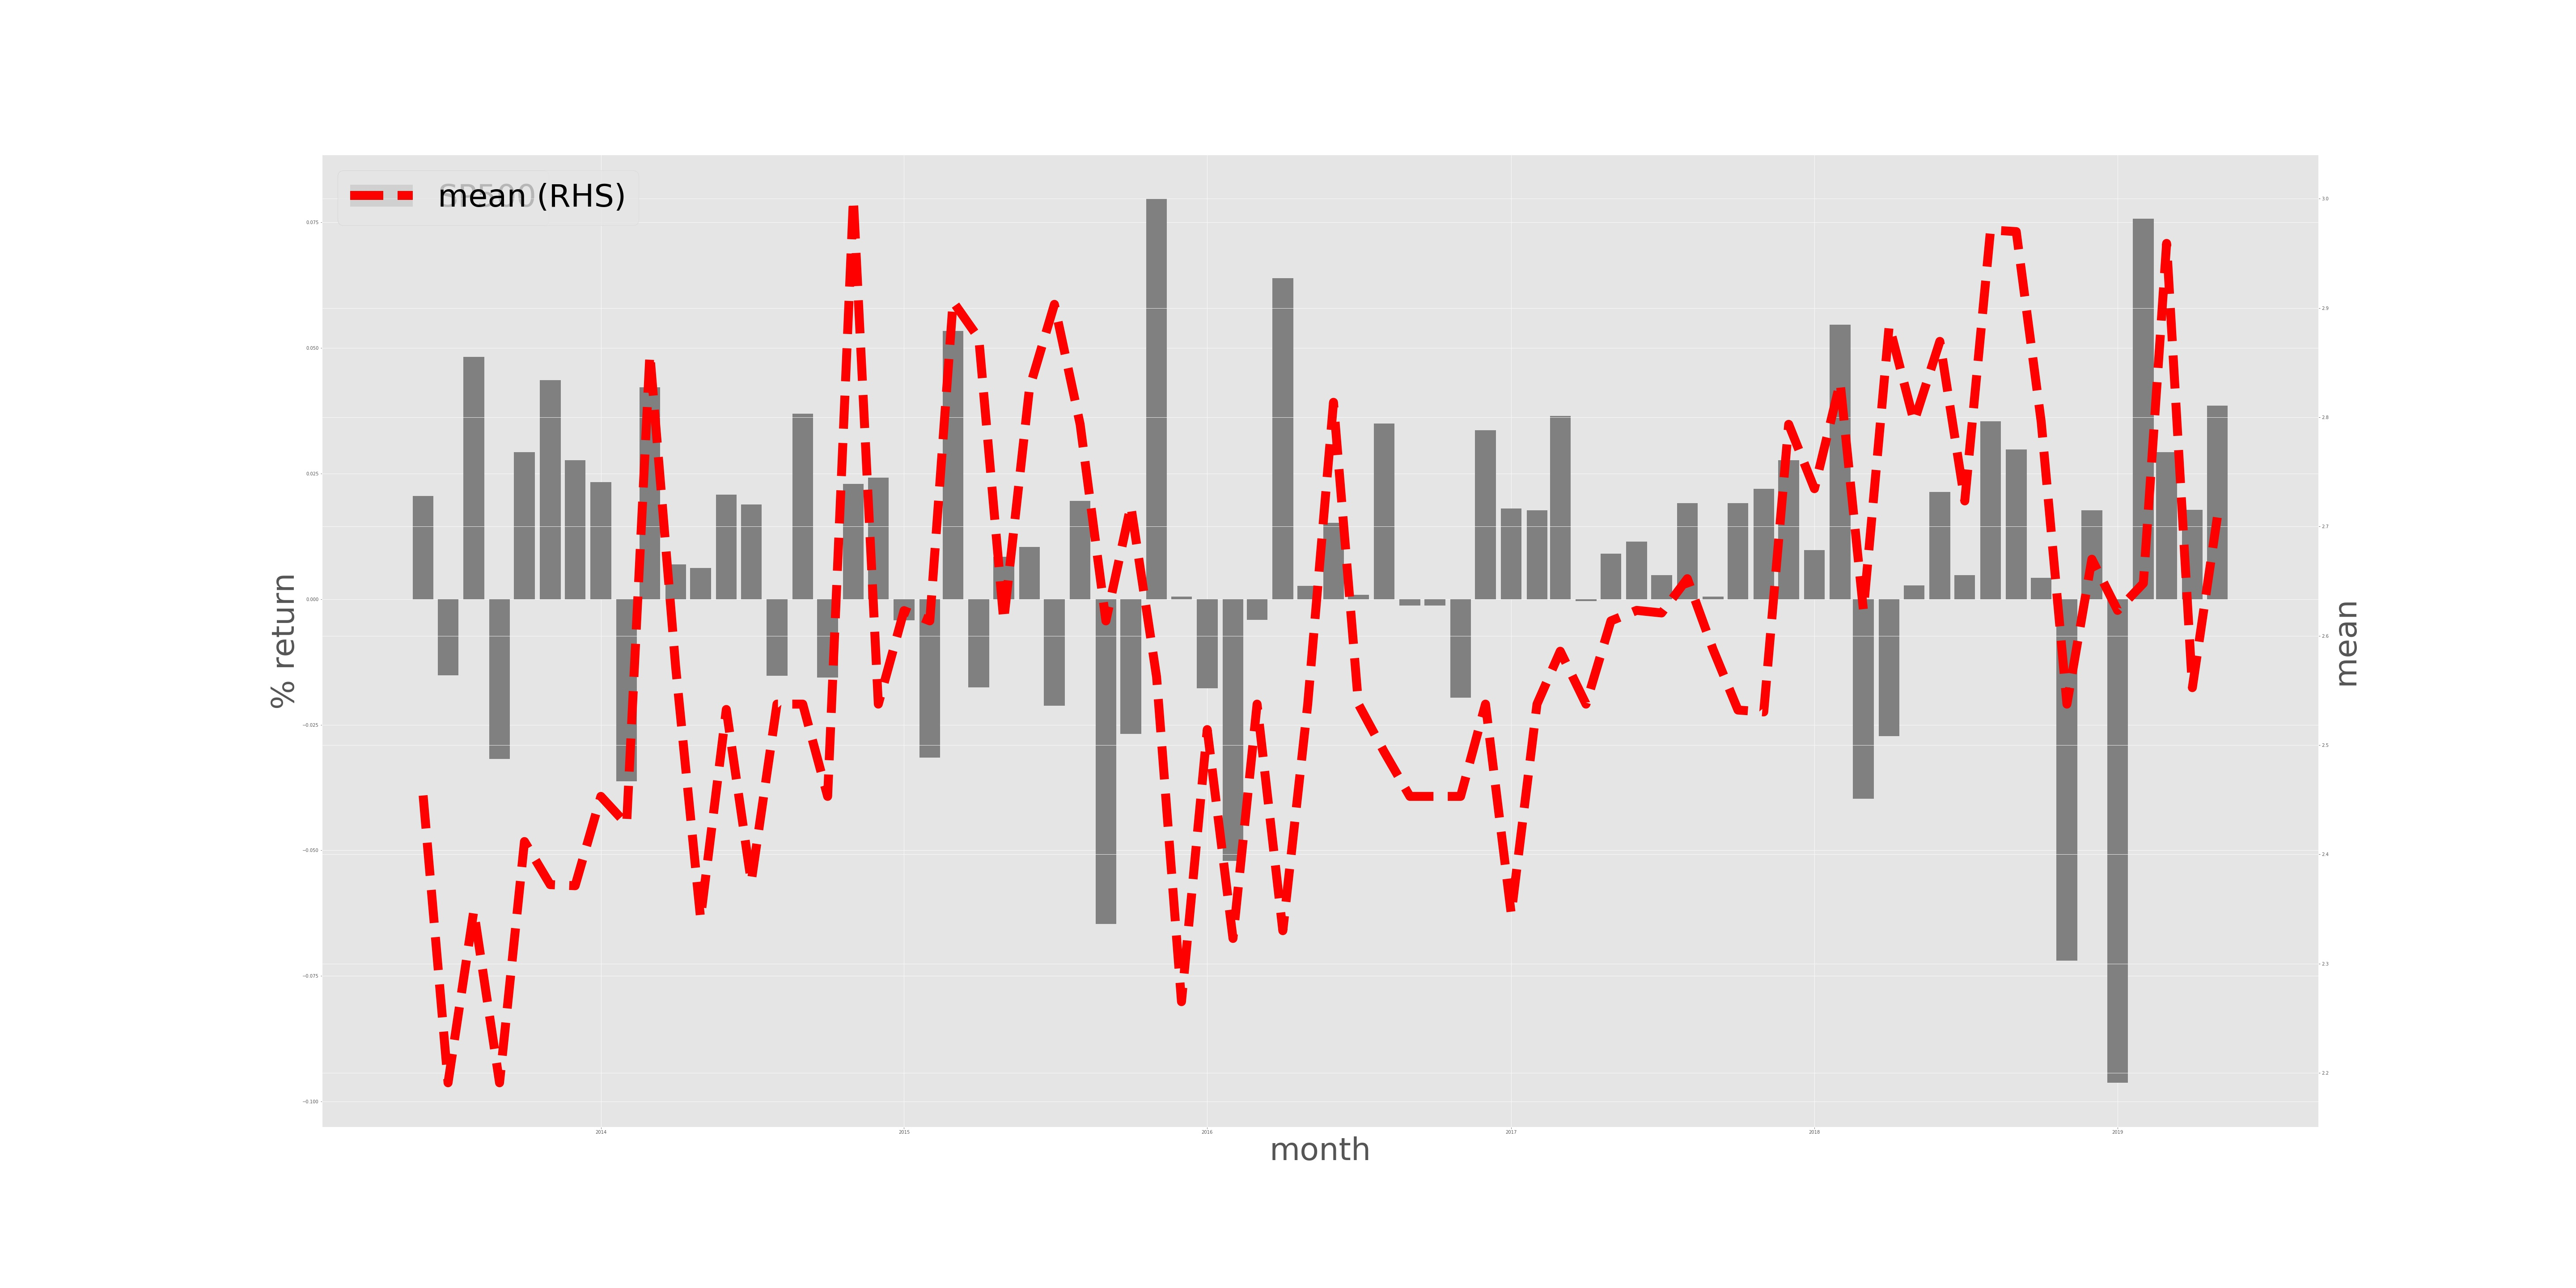
\includegraphics[width=\textwidth]{figures/tsMedmean.jpg}
	\end{figure}
	\begin{itemize}
		\item 
	\end{itemize}
\end{frame}


\begin{frame}{Dispersion risks and stock market performance}
	\begin{figure}
		\centering
		\label{ts_var}
		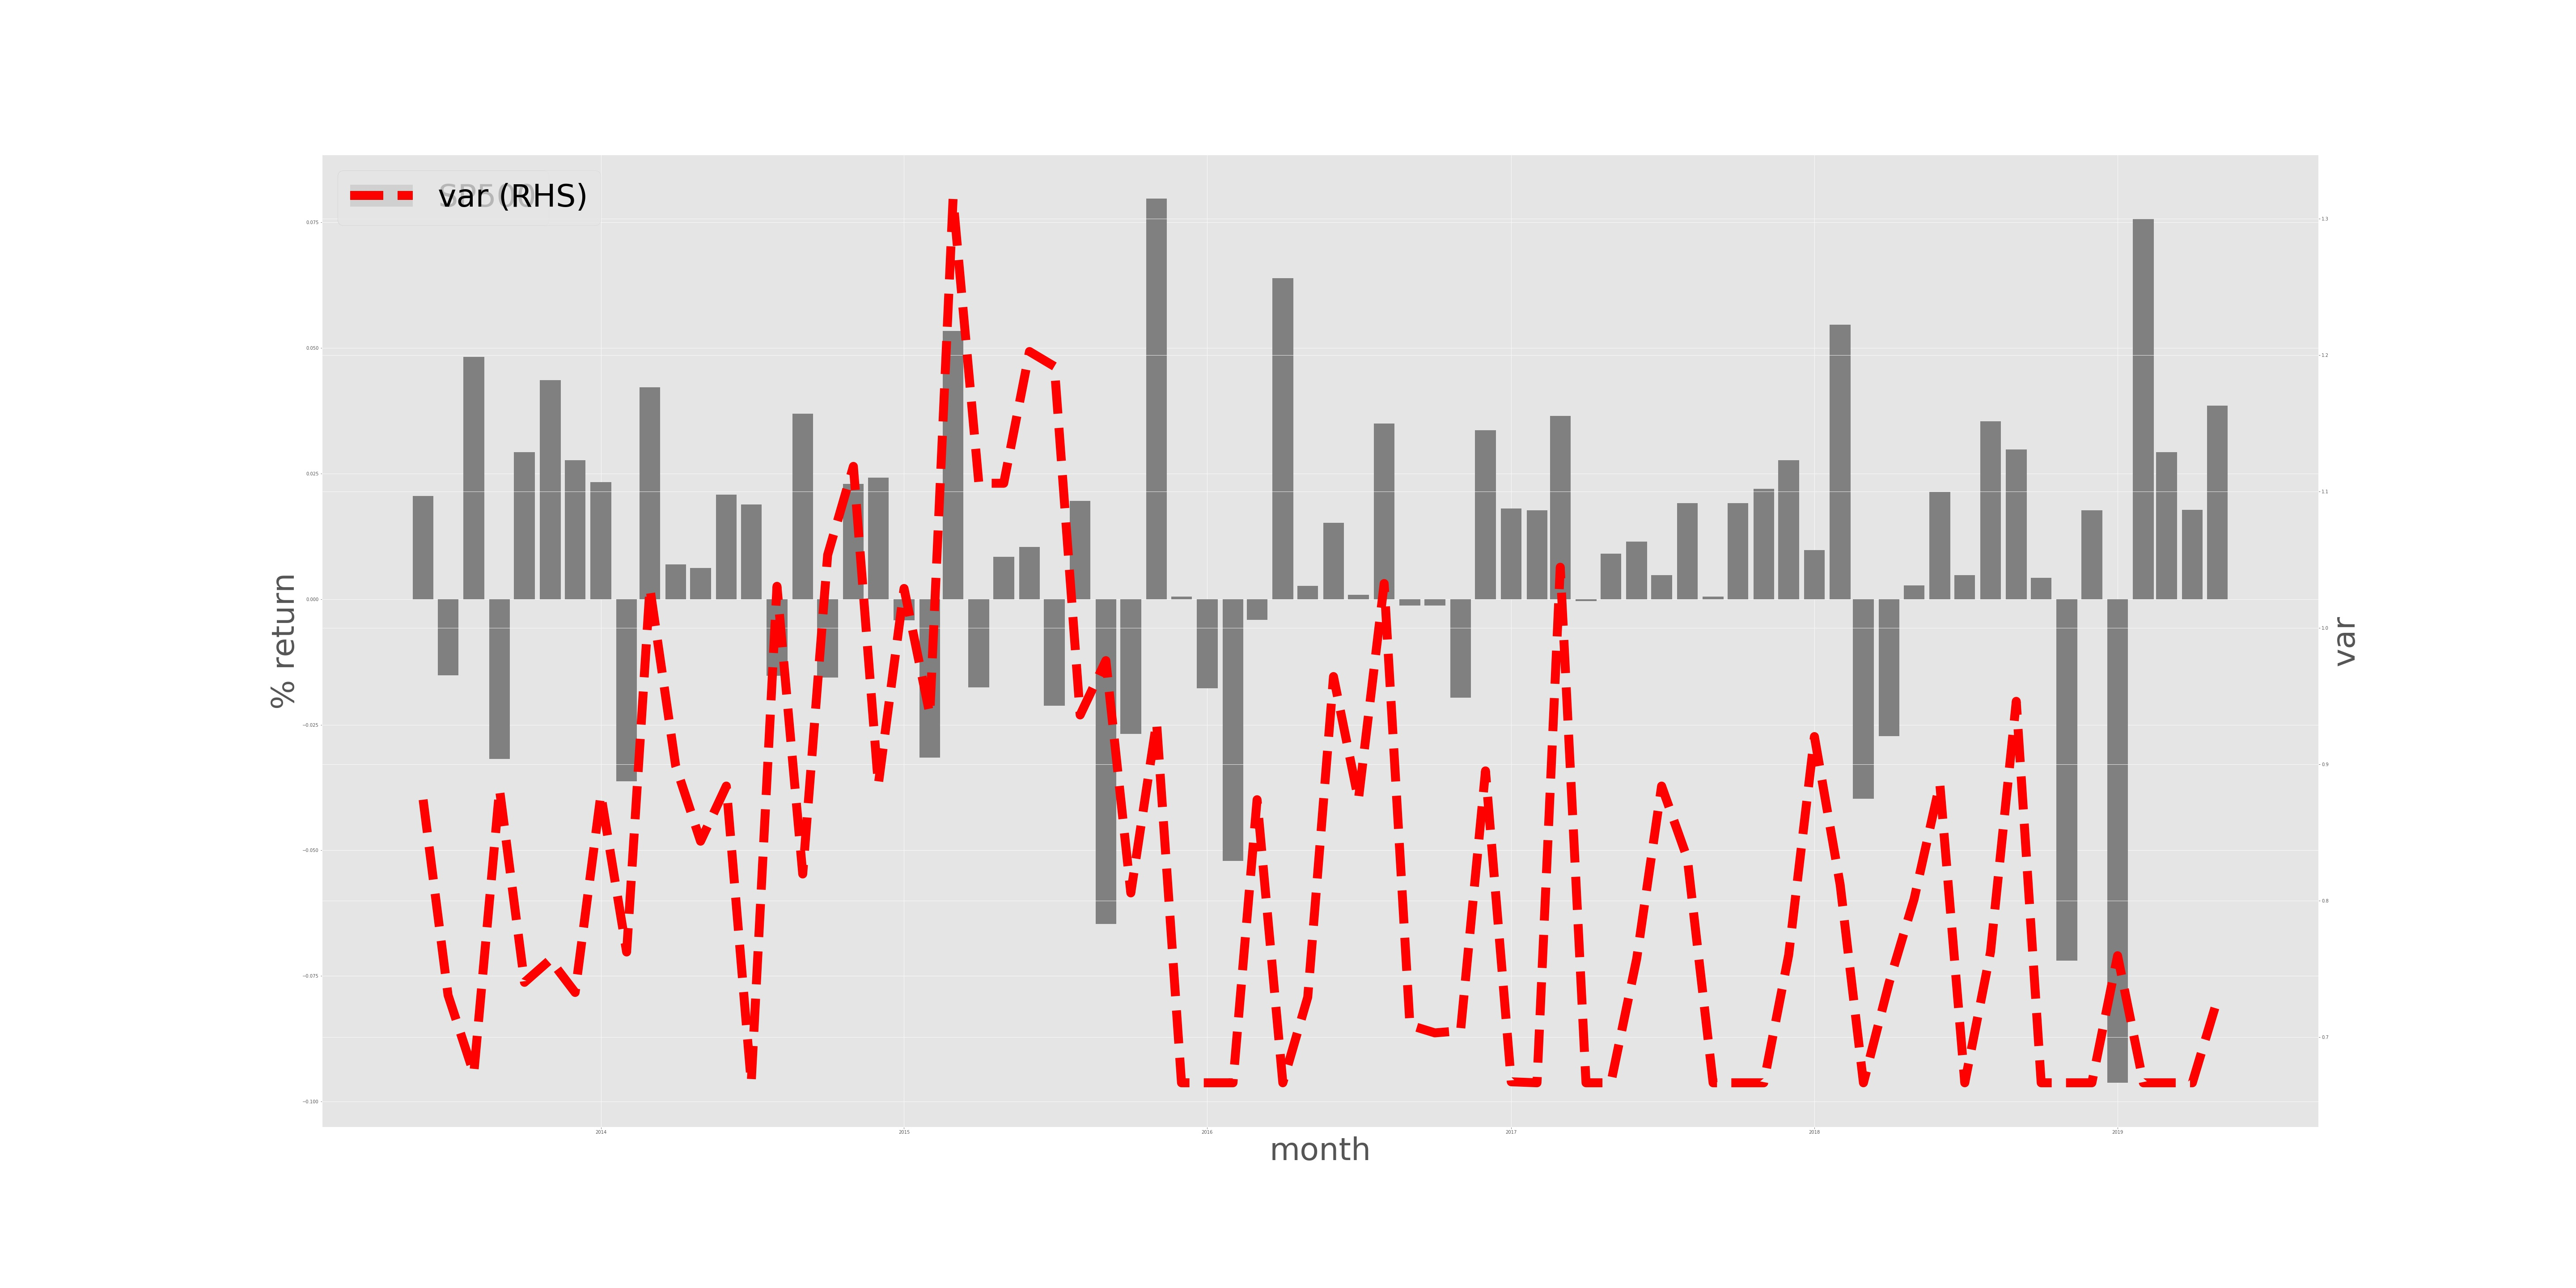
\includegraphics[width=\textwidth]{figures/tsMedvar.jpg}
	\end{figure}
	\begin{itemize}
		\item 
	\end{itemize}
\end{frame}



\begin{frame}{Tail risks and stock market performance}
	\begin{figure}
		\centering
		\label{ts_skew}
		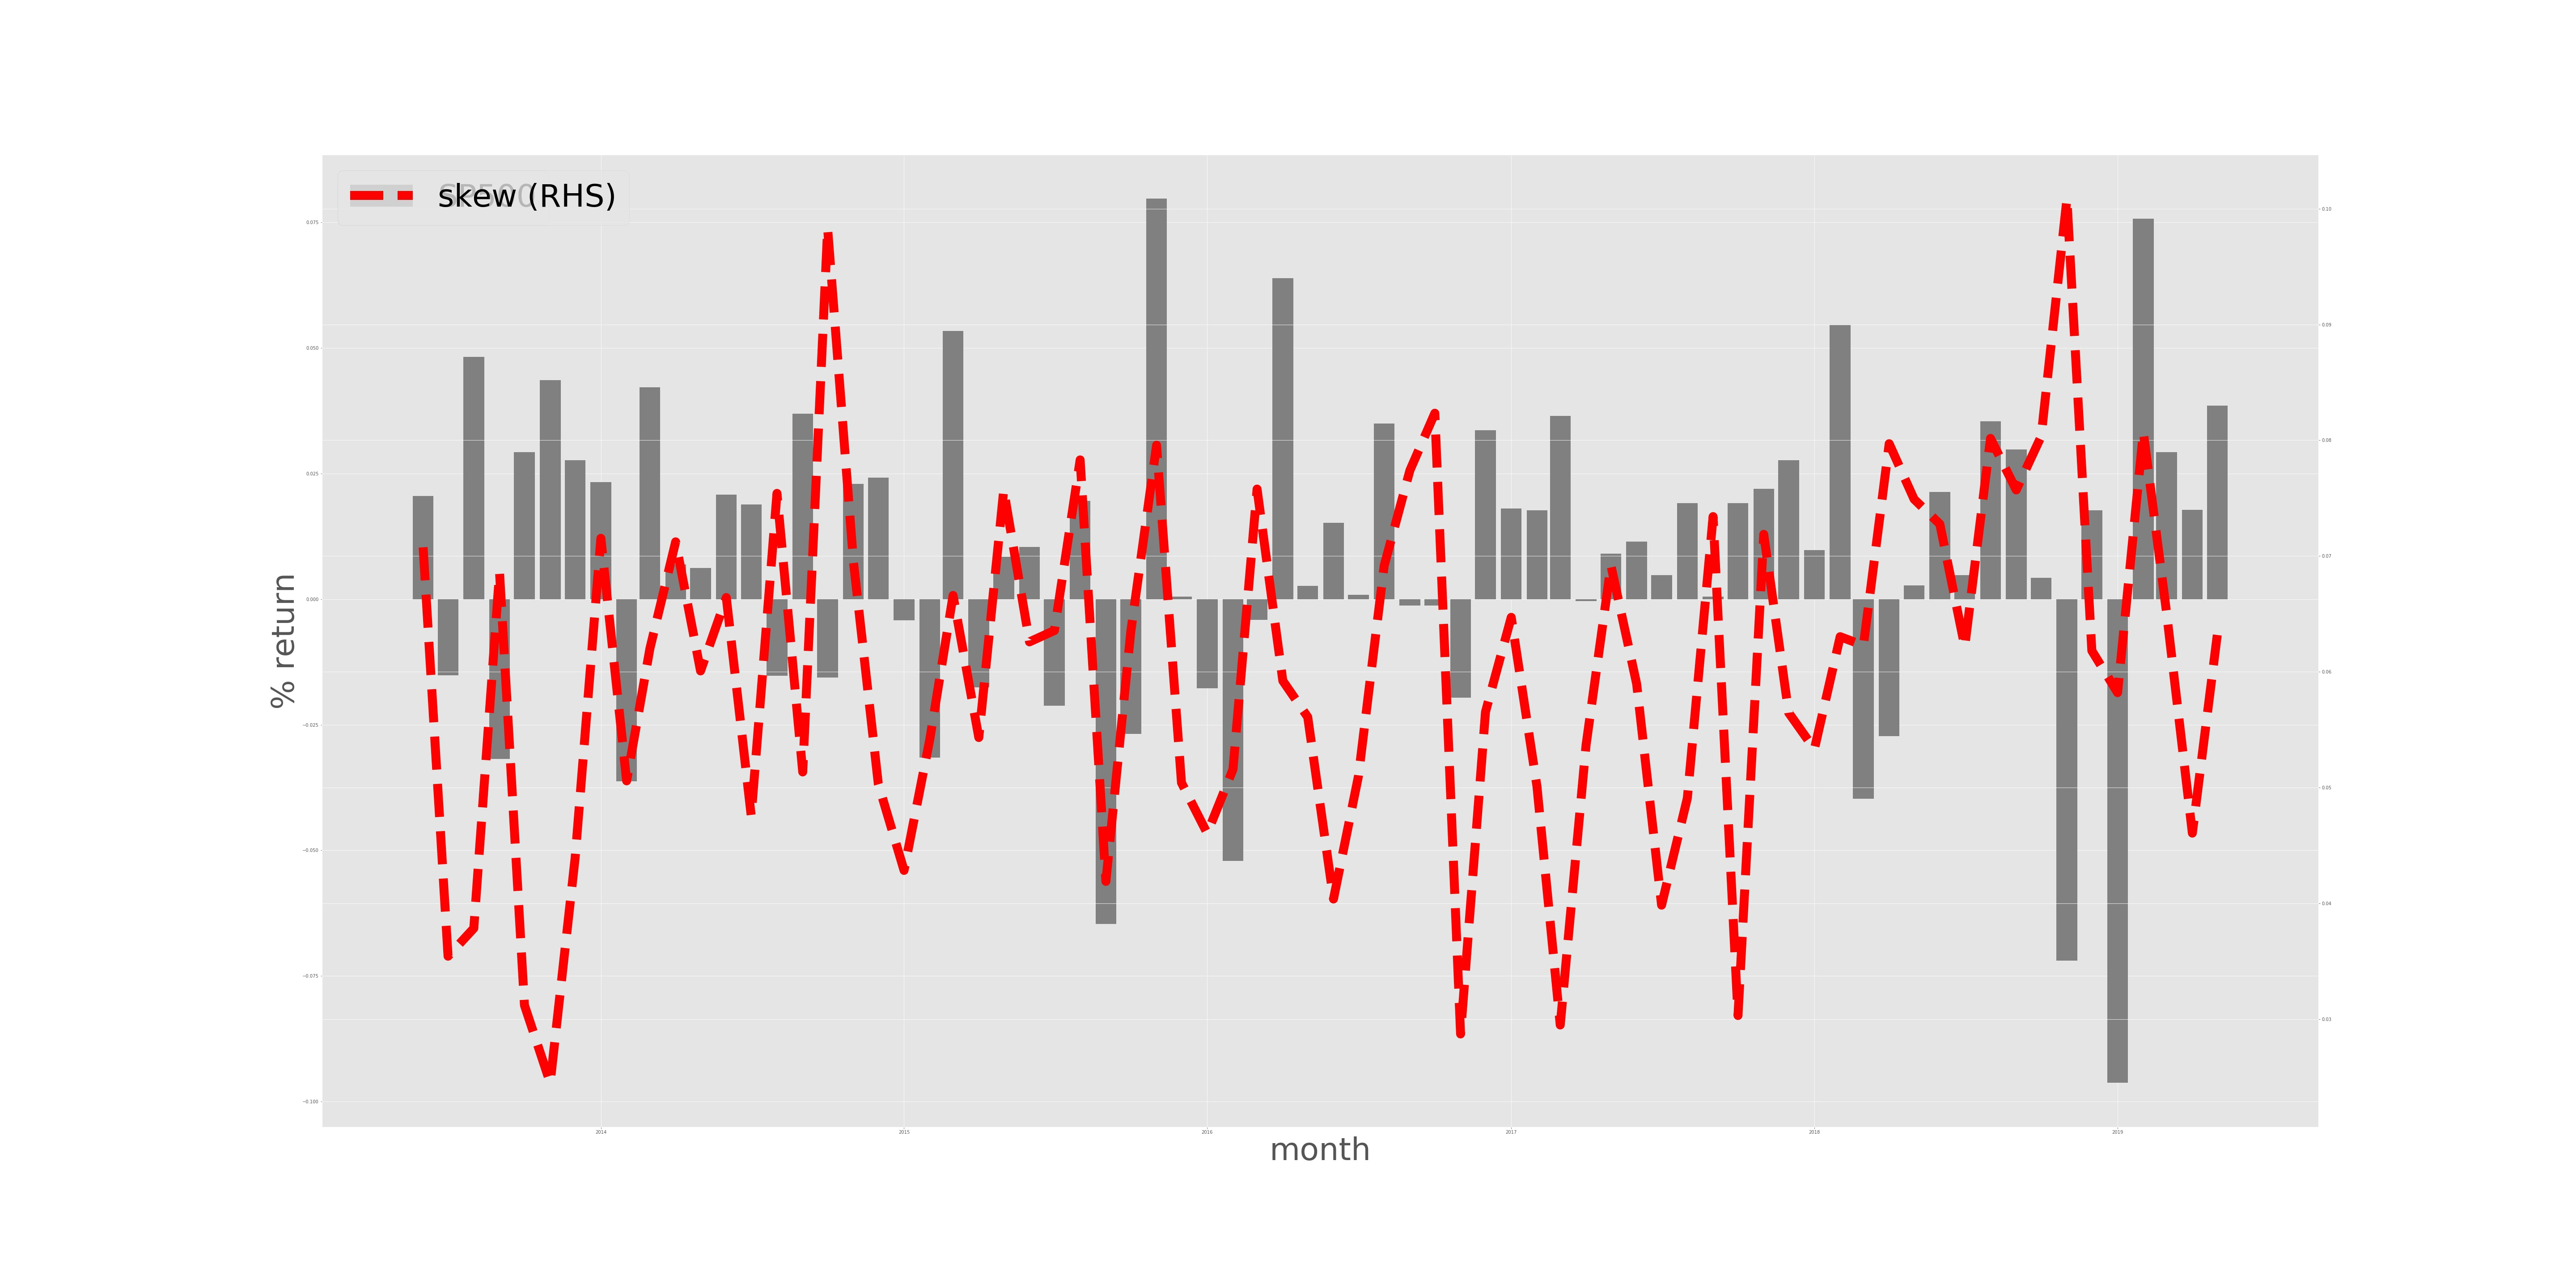
\includegraphics[width=\textwidth]{figures/tsEstMeanskew.jpg}
	\end{figure}
	\begin{itemize}
		\item 
	\end{itemize}
\end{frame}


\subsection{Permanent/transitory decomposition (work in progress)}

\begin{frame}{Underlying income process}
	
	\begin{itemize}
		\item Income of individual $i$, cohort $c$ at time $t$ 
		\begin{eqnarray*}
			\begin{split}
				& y_{i,c,t} = p_{i,c,t}+ \epsilon_{i,c,t},\quad \textrm{where } \epsilon_{i,c,t} \sim N(0,\sigma^2_{c,\epsilon}) \\
				& p_{i,c,t} = p_{i,c,t-1} + \theta_{i,c,t}, \quad \textrm{where }  \theta_{i,c,t} \sim N(0,\sigma^2_{\theta,c,t} ) \\
				& \log\sigma^2_{\theta,c,t} = \rho_c \log\sigma^2_{\theta,c,t-1} + \mu_{\theta,c,t}  \\
				& \mu_{\theta,c,t} \sim N(0,\gamma_c^2)
			\end{split}
		\end{eqnarray*}

	
		\item Parameters for cohort $c$
		\begin{itemize}
			\item $\rho_{c}$: how persistent is the innovation to the size of  the permanent risk  
			\item $\gamma_c$: how large is the innovation to the size of permanent risk
			\item $\sigma_{c,\epsilon}$: the time-invariant size of the transitory risk
		\end{itemize}
	\end{itemize}
\end{frame}


\begin{frame}{Perveived risk for 1-year-ahead growth}
	\begin{itemize}
		\item Under a perfect understanding of the income process
	\end{itemize}
	\begin{itemize}
		\item Perceived risks about next-month growth $\Delta y_{i,t}$
		\begin{eqnarray*}
			\begin{split}
				& \overline {var_{i,t}}(\Delta y_{i,t+1}) & = E_{i,t}( {\sigma^2_{\theta,t+1}}) + \sigma^2_{\epsilon} \\
				& & = \rho e^{-0.5\gamma} \sigma^2_{\theta,t}  + \sigma^2_{\epsilon} + \underbrace{\omega_{i,t}}_{\text{perception shock}}
			\end{split}
		\end{eqnarray*}
		
		\item Perceived risks about next-year growth $\Delta Y_{i,t}$
		\begin{eqnarray*}
		\begin{split}
			& \overline {var_{i,t}}(\Delta Y_{i,t+12}) \\
			& = \sum^{12}_{k=1} (12-k+1)^2 E_{i,t}( {\sigma^2_{\theta,t+k}}) + 12 \sigma^2_{\epsilon}  \\ 
			& = \sum^{12}_{k=1} (12-k+1)^2 \rho^k e^{-0.5k\gamma} \sigma^2_{\theta,t}+ 12 \sigma^2_{\epsilon} \\ 	 
		\end{split}
	\end{eqnarray*}
	\end{itemize}
\end{frame}

\begin{frame}{Perceived permanent and transitory decomposition}
	\begin{enumerate}
	\item Do GMM estimation using observed perceived risks from the data 
	\begin{itemize}
     \item Using average perceived risks, variance, autocovariance across the whole population or within specified cohort
	\end{itemize}
\item	With the estimated paramete, we will have a breakdown of the permanent and transitory risks. We can redo the exercises in previous sections seperately. 
\end{enumerate}
\end{frame}


\section{Model (work in progress)}

\begin{frame}{Model ingredients}
	
	\begin{enumerate}
		\item imperfect understanding of the income process, a deviation from rational expectation benchmark. 
		\begin{itemize}
			\item experience-based learning capturing the cross-generation and age-dependence income perceptions
		\end{itemize}
		\item a finite life cycle with a constant probability of death 
		\item uninsured idiosyncratic risks and aggregate risks (the workhorse assumption of the HANK literature) 
		\item single asset, i.e. no distinction between liquid and iliquid assets 
	\end{enumerate}
\end{frame}

\begin{frame}{Intuitions behind the model mechanisms}
	\begin{itemize}
		\item an imperfect understanding $ \quad \rightarrow$ heterogeneous perception of risks $ \quad \text{AND } $ uninsurance of risks $ \quad \rightarrow$ difference in precautionary motives and MPCs across populations $ \quad \rightarrow$ potential amplification of aggregate MPC
	\end{itemize}
\end{frame}

%%%%%%%%%%%%%%%%%%%


%%%%%%%%%%%%%%%%%%%%%%%%%%%%%%%%%


\section{Conclusion}

\begin{frame}{Conclusion}
	\begin{itemize}
		\item ddddd
	\end{itemize}	
\end{frame}

\section*{Appendix}

\begin{frame}{Density estimation and robustness of my results}
	\begin{itemize}
		\item ddd
	\end{itemize}
\end{frame}


\bibliographystyle{apalike}
\bibliography{PerceivedIncomeRisk}


\end{document}
